% Extracted from SupplementaryMaterials_ExperimentAudit.tex for the combined arXiv manuscript.

In this appendix, we provide technical details and more comprehensive analyses
of our proposed method. It comprises Section~\ref{app:backbone},
\emph{Backbone, Algorithm and Hyperparameters};
Section~\ref{app:visual-quality-feature-analysis},
\emph{Visual Quality Feature Analysis}; Section~\ref{app:editor-proxy},
\emph{Discussion on the Editor Proxy}; and
Section~\ref{app:credit-mask-audit}, \emph{Detailed Credit-Mask Audit}.
\section{Backbone, Algorithm and Hyperparameters}
\label{app:backbone}

\subsection{Dataset Protocol.}
Our training and evaluation settings follow the same configuration as the main
paper. We train on the KonIQ-10k training subset~\citep{koniq} and use a fixed
set of 200 images randomly sampled from the KonIQ-10k test split to monitor
early-stage convergence. Final testing is conducted on the KonIQ-10k test
split, SPAQ~\citep{spaq}, LIVE-W~\citep{live-w},
AGIQA-3K~\citep{agiqa}, KADID-10k~\citep{kadid}, and CSIQ~\citep{csiq}.

At the time of manuscript completion, we did not have access to
Zoom-IQA~\citep{zoom-iqa} and therefore could not reproduce it under our
protocol. Tool-IQA~\citep{tool-iqa} follows a different training--testing
configuration; consequently, we cannot report directly comparable Tool-IQA
results for some experiments.

For the cross Actor--Judge--Editor evaluation reported in Table~2 of the main
paper, we use a fixed 5,866-image subset, randomly sampling 1,000 images from
each test set except CSIQ, for which all 866 images are used. This subsampling
is necessary for computational efficiency: evaluating the full test sets would
involve approximately 23,000 images, each requiring four editing operations
and three Judge evaluations, resulting in a prohibitively heavy inference
cost.

\subsection{Candidate Backbones.}
The Qwen series has been widely adopted in recent BIQA studies due to its open-source availability, strong multimodal capability, and computational efficiency.
For example, existing methods such as Q-Insight~\citep{q-insight},
VQ-R1~\citep{Visualquality-r1}, and Zoom-IQA~\citep{zoom-iqa} employ
Qwen2.5-VL-7B~\citep{qwen2.5} as their backbone model.
However, despite its strong performance, the 7B-scale model still introduces considerable computational overhead, which limits its practical deployment and training efficiency.

Therefore, in this work, we investigate more lightweight backbone configurations with 2B and 4B parameters.
Considering future scalability and the continuous evolution of multimodal large language models, we further evaluate the latest Qwen3-VL and Qwen3.5-VL architectures.
We conduct comprehensive backbone comparisons among 2B/4B variants of Qwen3 and Qwen3.5 to identify an optimal trade-off between training efficiency and performance.

\paragraph{Qwen3-VL versus Qwen3.5.}
The T1--T2 comparison in Table~\ref{tab:preliminary-ablation} shows that, under
matched frozen-vision DAPO settings, Qwen3.5-2B outperforms Qwen3-VL-2B on five
of six datasets for both PLCC and SRCC, and on all six in MAE. It also requires
only 0.81$\times$ the training time per epoch.

\paragraph{2B versus 4B.}
The T6--T7 comparison in Table~\ref{tab:preliminary-ablation} shows that the 4B
model converges faster in rating performance. By Epoch 2, T7 reaches a
validation PLCC/SRCC/MAE of
0.929/0.919/0.566, compared with 0.915/0.904/0.744 for the 2B T6; by Epoch 3,
T7 further improves to 0.935/0.924/0.228. The 4B model also produces more
diverse outputs, with 83 distinct ratings, 200 unique completions, and a
41.5\% U-score, compared with a 39.0\% U-score for T6. We further observe that
its response lengths are better aligned with our objective of eliciting
detailed quality reasoning.

\begin{table*}[!t]
\centering
{\small
\setlength{\tabcolsep}{4.5pt}
\begin{tabular}{@{}lcrccr@{}}
\toprule
\textbf{Variant} & \textbf{Iter.} & \textbf{Time (h/ep.)} &
\textbf{Val. P/S/M} & \textbf{U-score (\%)} & \textbf{Gen. P/S/M} \\
\midrule
\multicolumn{6}{@{}l}{\emph{(a) Qwen3-VL-2B}} \\
T1: DAPO i1, frozen, global & 1 & 1.38 & 0.831/0.817/0.868 & 12.0 & 0.809/0.787/0.936 \\
\addlinespace[1pt]
\multicolumn{6}{@{}l}{\emph{(b) Qwen3.5-2B}} \\
T2: DAPO i1, frozen, global & 1 & 1.13 & 0.890/0.881/0.691 & 36.0 & \textbf{0.835}/0.808/0.740 \\
T3: DAPO i4, frozen, global & 4 & 2.47 & 0.910/0.904/0.265 & 21.5 & 0.834/0.809/0.541 \\
T4: GRPO i1, frozen & 1 & 0.81 & 0.886/0.883/0.845 & 34.0 & 0.829/0.800/0.878 \\
T5: DAPO i1, visual, global & 1 & 1.30 & \textbf{0.929}/\textbf{0.921}/\textbf{0.261} & 35.0 & 0.828/0.809/\textbf{0.513} \\
T6: DAPO i1, visual, local-six & 1 & 1.54 & 0.917/0.906/0.587 & 39.0 & \textbf{0.835}/\textbf{0.813}/0.684 \\
\addlinespace[1pt]
\multicolumn{6}{@{}l}{\emph{(c) Qwen3.5-4B, local-six}} \\
T7: DAPO i1, visual, local-six & 1 & 2.56 & 0.935/0.924/0.228 & 41.5 & -- \\
\bottomrule
\end{tabular}
}
\caption{Actor-only ablations at their reported endpoints.
$\mathrm{P}/\mathrm{S}/\mathrm{M}$ denotes PLCC/SRCC/MAE; Val. is the aligned
200-image set, and Gen. is the six-dataset macro average. U-score measures
distinct validation ratings, and Time is the mean wall-clock time per epoch.
Bold marks the best alignment result among the controlled Qwen3.5-2B variants;
higher PLCC/SRCC and lower MAE are better. All variants use E3.}
\label{tab:preliminary-ablation}
\end{table*}

\begin{figure*}[!t]
\centering
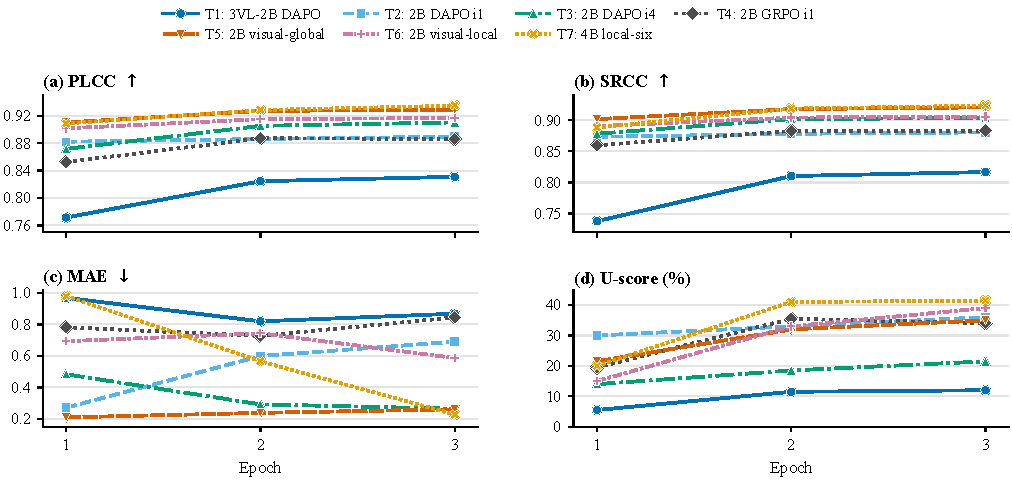
\includegraphics[width=\textwidth]{Figures/fig_ablation_epochs}
\caption{Validation trajectories through E3 on the common 200-image set. T7
denotes the 4B local-six run. Curves are single fixed-seed runs, so no error
bands are shown. Higher PLCC/SRCC and
lower MAE are better, while U-score diagnoses rating diversity. Color, marker,
and line style consistently identify T1--T7.}
\label{fig:ablation-epochs}
\end{figure*}

\begin{figure*}[!t]
\centering
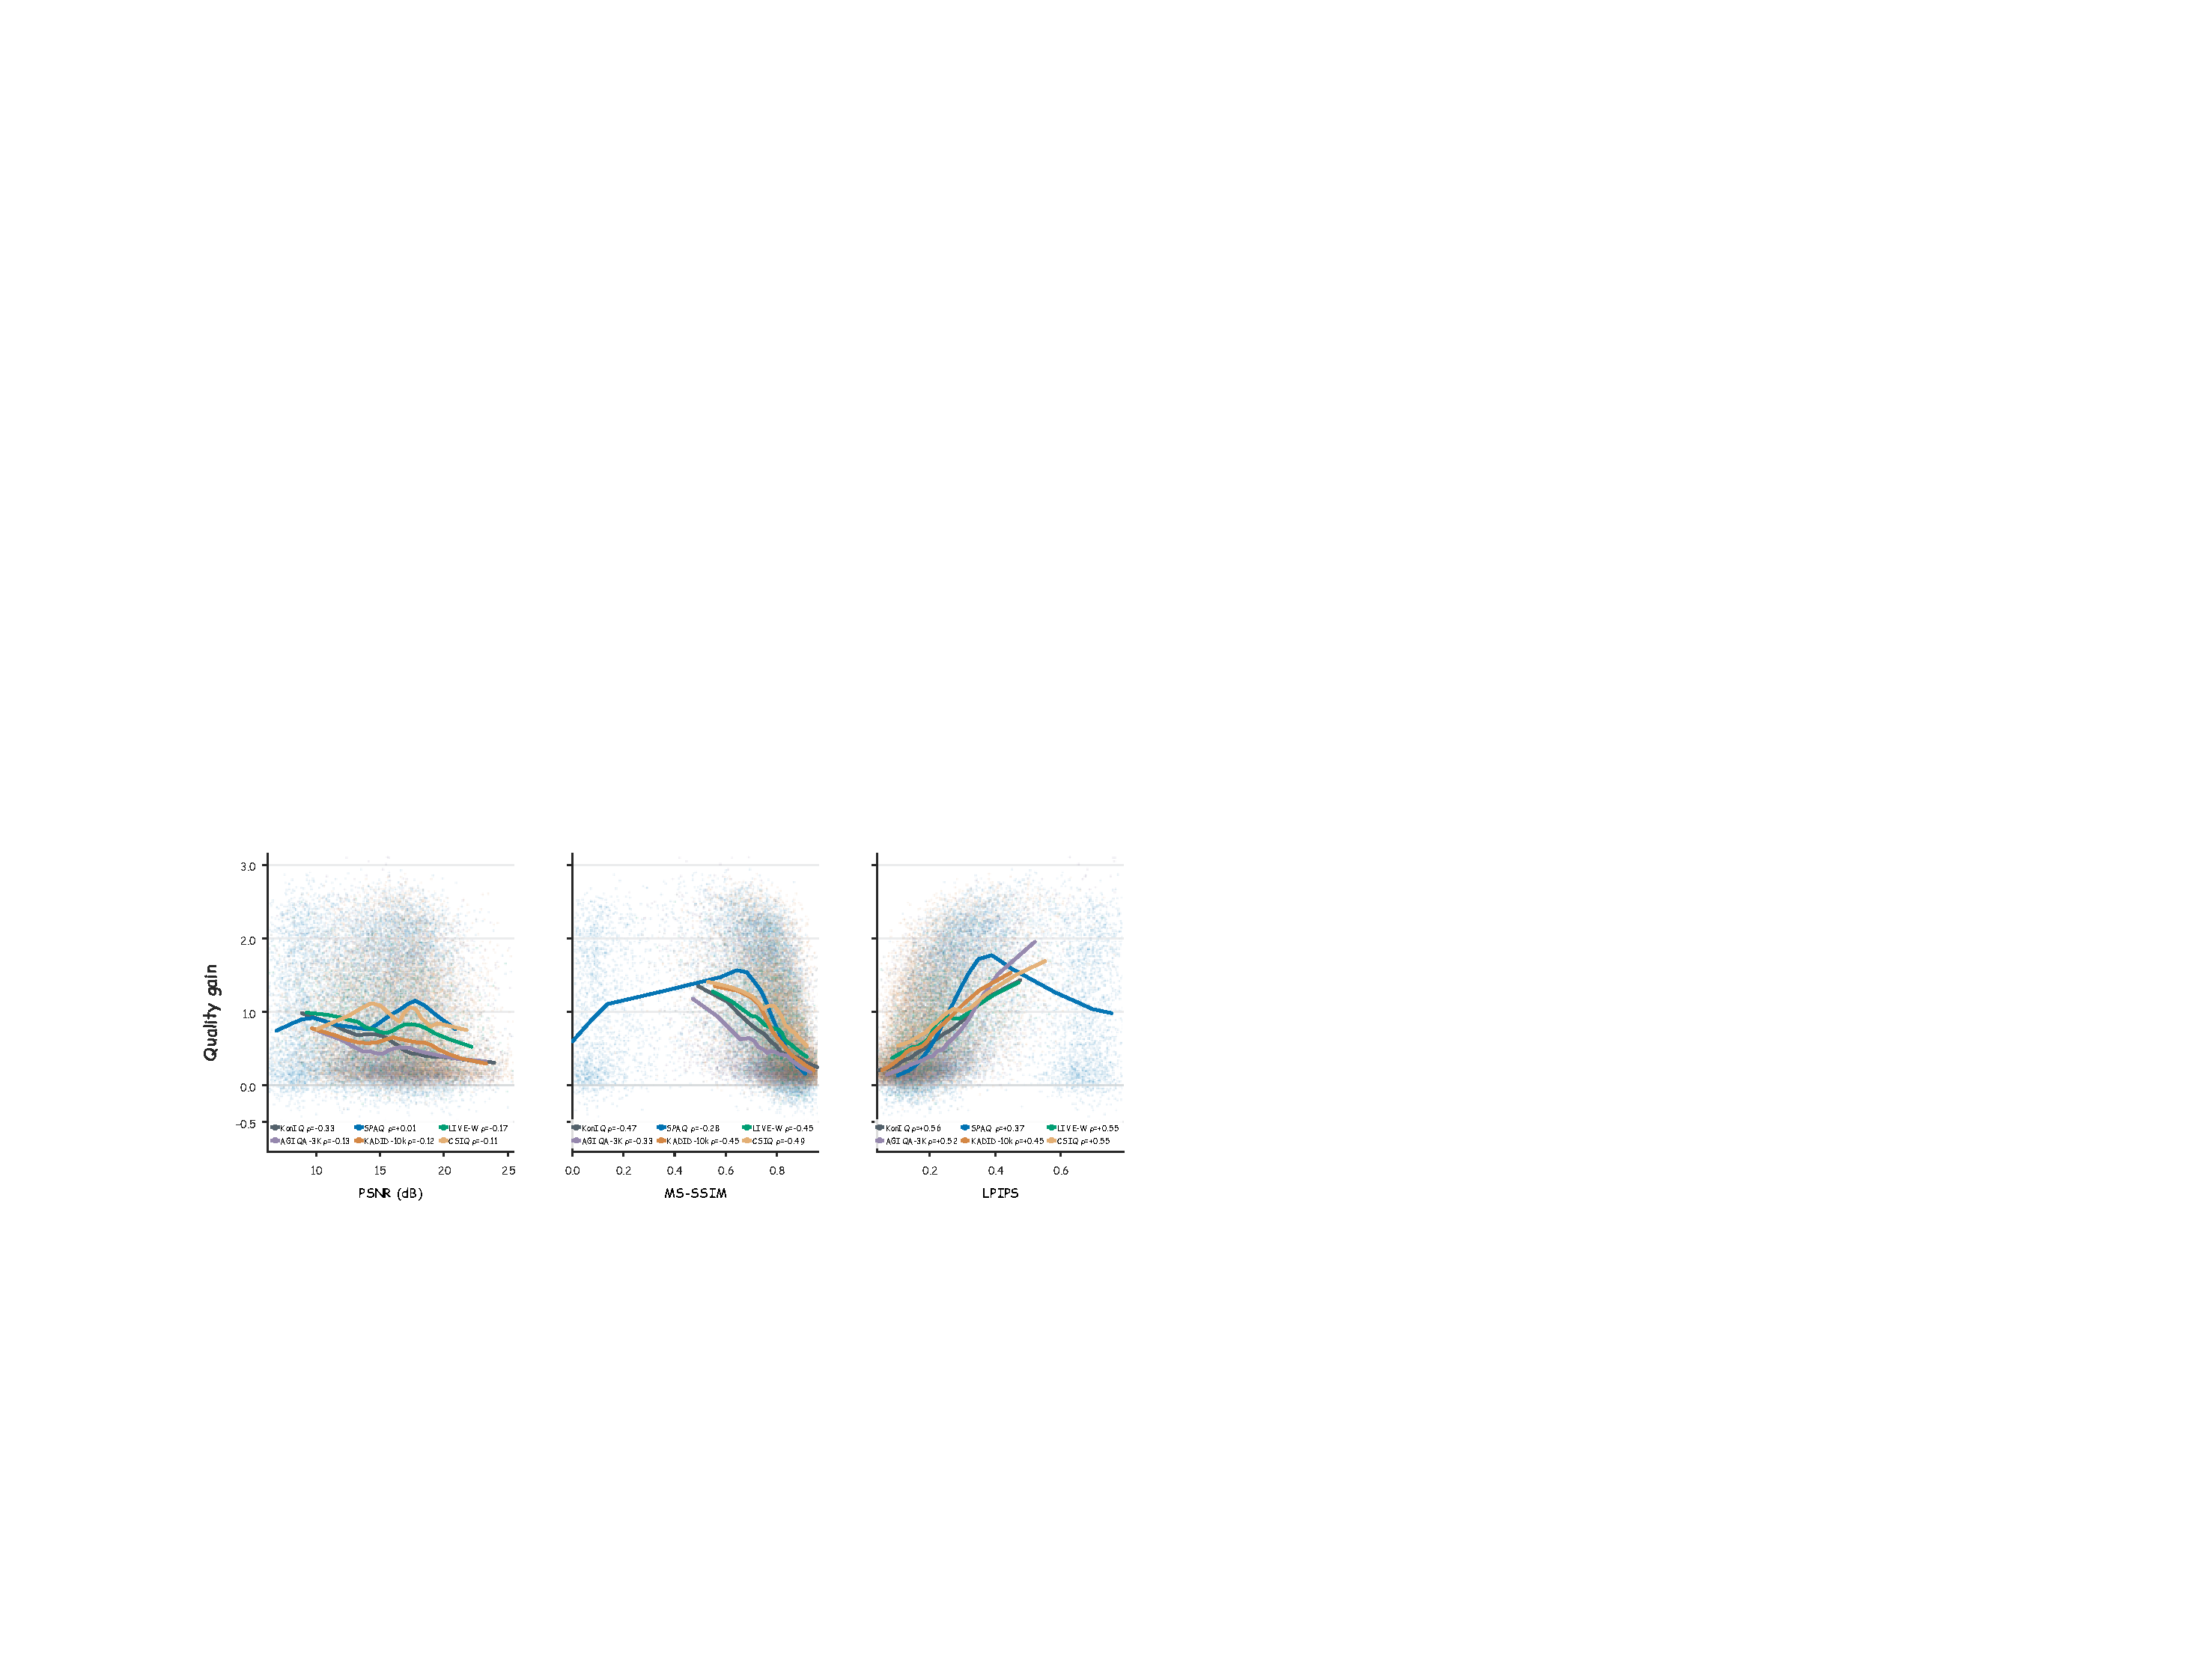
\includegraphics[width=\textwidth]{Figures/af2_analysis}
\caption{\textbf{Quality gain versus visual change scale.}
The panels relate the Judge-observed quality gain $\Delta s$ to PSNR,
MS-SSIM~\citep{wang2003msssim}, and LPIPS~\citep{zhang2018lpips} between the
original and edited images. Colors denote datasets, curves show smoothed
trends, and $\rho$ denotes Spearman correlation.}
\label{fig:quality-fidelity}
\end{figure*}

\subsection{Optimization Algorithms: GRPO or DAPO?}
\label{app:optimization-algorithms}

Compared with GRPO~\citep{shao2024deepseekmath},
DAPO~\citep{yu2025dapo} dynamically resamples low-variance groups, thereby
increasing within-group reward diversity and preventing policy advantages from
vanishing prematurely. We therefore adopted DAPO in most of our early
experiments.

Across three epochs, 3,282 of 20,832 GRPO learner groups (15.75\%) have zero
within-group reward variance and therefore zero policy advantage. DAPO
resampling reduces the proportion of zero-advantage learner groups to 0\%.
Comparing T2 and T4 in Table~\ref{tab:preliminary-ablation}, DAPO improves
the six-dataset macro PLCC/SRCC by 0.006/0.008 and reduces MAE by 0.138 at
Epoch 3, with improvements on five, six, and six datasets, respectively.

Despite its better performance, DAPO requires 1.866$\times$ more sampled
trajectories and increases the training time per epoch from 0.81 to 1.13 hours
(approximately 39.5\%). This additional training-time cost is
not affordable in our training environment, especially when scaling the model
to 4B parameters or beyond. Therefore, we use GRPO as the default optimization
algorithm in the final framework.

\subsection{Hyper-Parameter Settings.}

\paragraph{Group Size: 6 versus 48.}
MR-IQA~\citep{mr-iqa} reports its best performance with local groups of six,
where rewards are computed by comparing samples only within each six-image
group. Table~\ref{tab:preliminary-ablation} compares this local-6 setting (T6)
with a larger group of 48 (T5).
The large group achieves better in-domain validation PLCC/SRCC/MAE
(0.929/0.921/0.261 versus 0.917/0.906/0.587), whereas local-6 achieves higher
six-dataset macro PLCC/SRCC (0.835/0.813 versus 0.828/0.809). Because the
local-6 setting provides stronger cross-dataset correlation, we adopt a group
size of six.

\paragraph{Vision Modules: Frozen versus Active.}
The T2--T5 comparison in Table~\ref{tab:preliminary-ablation} shows that active
visual training performs better on authentic datasets, achieving
PLCC/SRCC values of 0.952/0.938 on KonIQ and 0.897/0.877 on LIVE-W, compared
with 0.925/0.904 and 0.881/0.847 for the frozen variant. In contrast, freezing
the vision encoder and aligner performs better on AGIQA-3K and the synthetic
datasets: it achieves 0.826/0.768 on AGIQA-3K, 0.665/0.676 on KADID-10k, and
0.840/0.801 on CSIQ, compared with 0.816/0.747, 0.661/0.668, and 0.771/0.746
under active visual training. Consequently, the frozen variant yields higher
six-dataset average PLCC/SRCC (0.840/0.816 versus 0.833/0.812), indicating
stronger overall generalization.

\paragraph{Rating Diversity.}
Zoom-IQA~\citep{zoom-iqa} reports score-space collapse when using a ranking
reward, with only a 2.04\% unique-score ratio. Across T1--T7 in
Table~\ref{tab:preliminary-ablation}, the E3 U-scores remain between 12.0\% and
41.5\%, corresponding to 24--83 distinct ratings on the 200-image validation
set. Thus, we do not observe rating-diversity collapse under our current
settings.

\paragraph{Repeated Sampling Updates.}
MR-IQA~\citep{mr-iqa} reuses each rollout sample for four policy updates. We
evaluate whether these repeated updates remain effective by comparing T2 and
T3 in Table~\ref{tab:preliminary-ablation}. Four updates improve validation
PLCC/SRCC/MAE from 0.890/0.881/0.691 to
0.910/0.904/0.265. However, the six-dataset macro PLCC/SRCC remain nearly
unchanged (0.835/0.808 versus 0.834/0.809), while training time increases from
1.13 to 2.47 hours per epoch. Therefore, one policy update per rollout is
sufficient under our current settings.

\section{Visual Quality Feature Analysis}
\label{app:visual-quality-feature-analysis}

In our framework, the FLUX.2 [klein] Editor~\citep{flux2} produces an edited
image conditioned on the quality reasoning for each input. The resulting
original--edited pair bridges single-image quality assessment with
reference-based quality assessment, enabling us to analyze how the visual
intervention relates to the predicted quality improvement. In this section, we
investigate three questions: (1) whether larger visual changes lead to greater
quality gains; (2) how the distributions of low-level visual features change
after editing; and (3) what behavioral preferences emerge from the overall
framework.

\subsection{Visual Change and Quality Gains}
\label{app:quality-fidelity}

\paragraph{Visual change and quality improvement.}
Figure~\ref{fig:quality-fidelity} relates the Judge-observed quality gain to
three reference-based measures of the visual change between the original and
edited images. Quality gain is generally negatively correlated with PSNR
($\rho=-0.33$ to $+0.01$) and MS-SSIM ($\rho=-0.49$ to $-0.28$), and
positively correlated with LPIPS ($\rho=0.37$ to $0.56$). Because larger
changes correspond to lower
PSNR/MS-SSIM and higher LPIPS, these consistent directions indicate that
larger editing changes are generally associated with greater image-quality
improvements. SPAQ deviates from the other datasets across multiple measures. Its
quality-gain correlation is nearly zero for PSNR ($\rho=+0.01$) and is the
weakest in magnitude for both MS-SSIM ($\rho=-0.28$) and LPIPS
($\rho=+0.37$). A similar pattern appears in rating performance: while the
rating correlations on the other datasets change during training, the SPAQ
correlation remains close to 0.90 with only minor variation. This stability
suggests that SPAQ is less sensitive to the training-induced changes observed
on the other benchmarks.

\subsection{Low-Level Visual Feature Patterns}
\label{app:quality-low-level-features}

\begin{figure*}[t!]
\centering
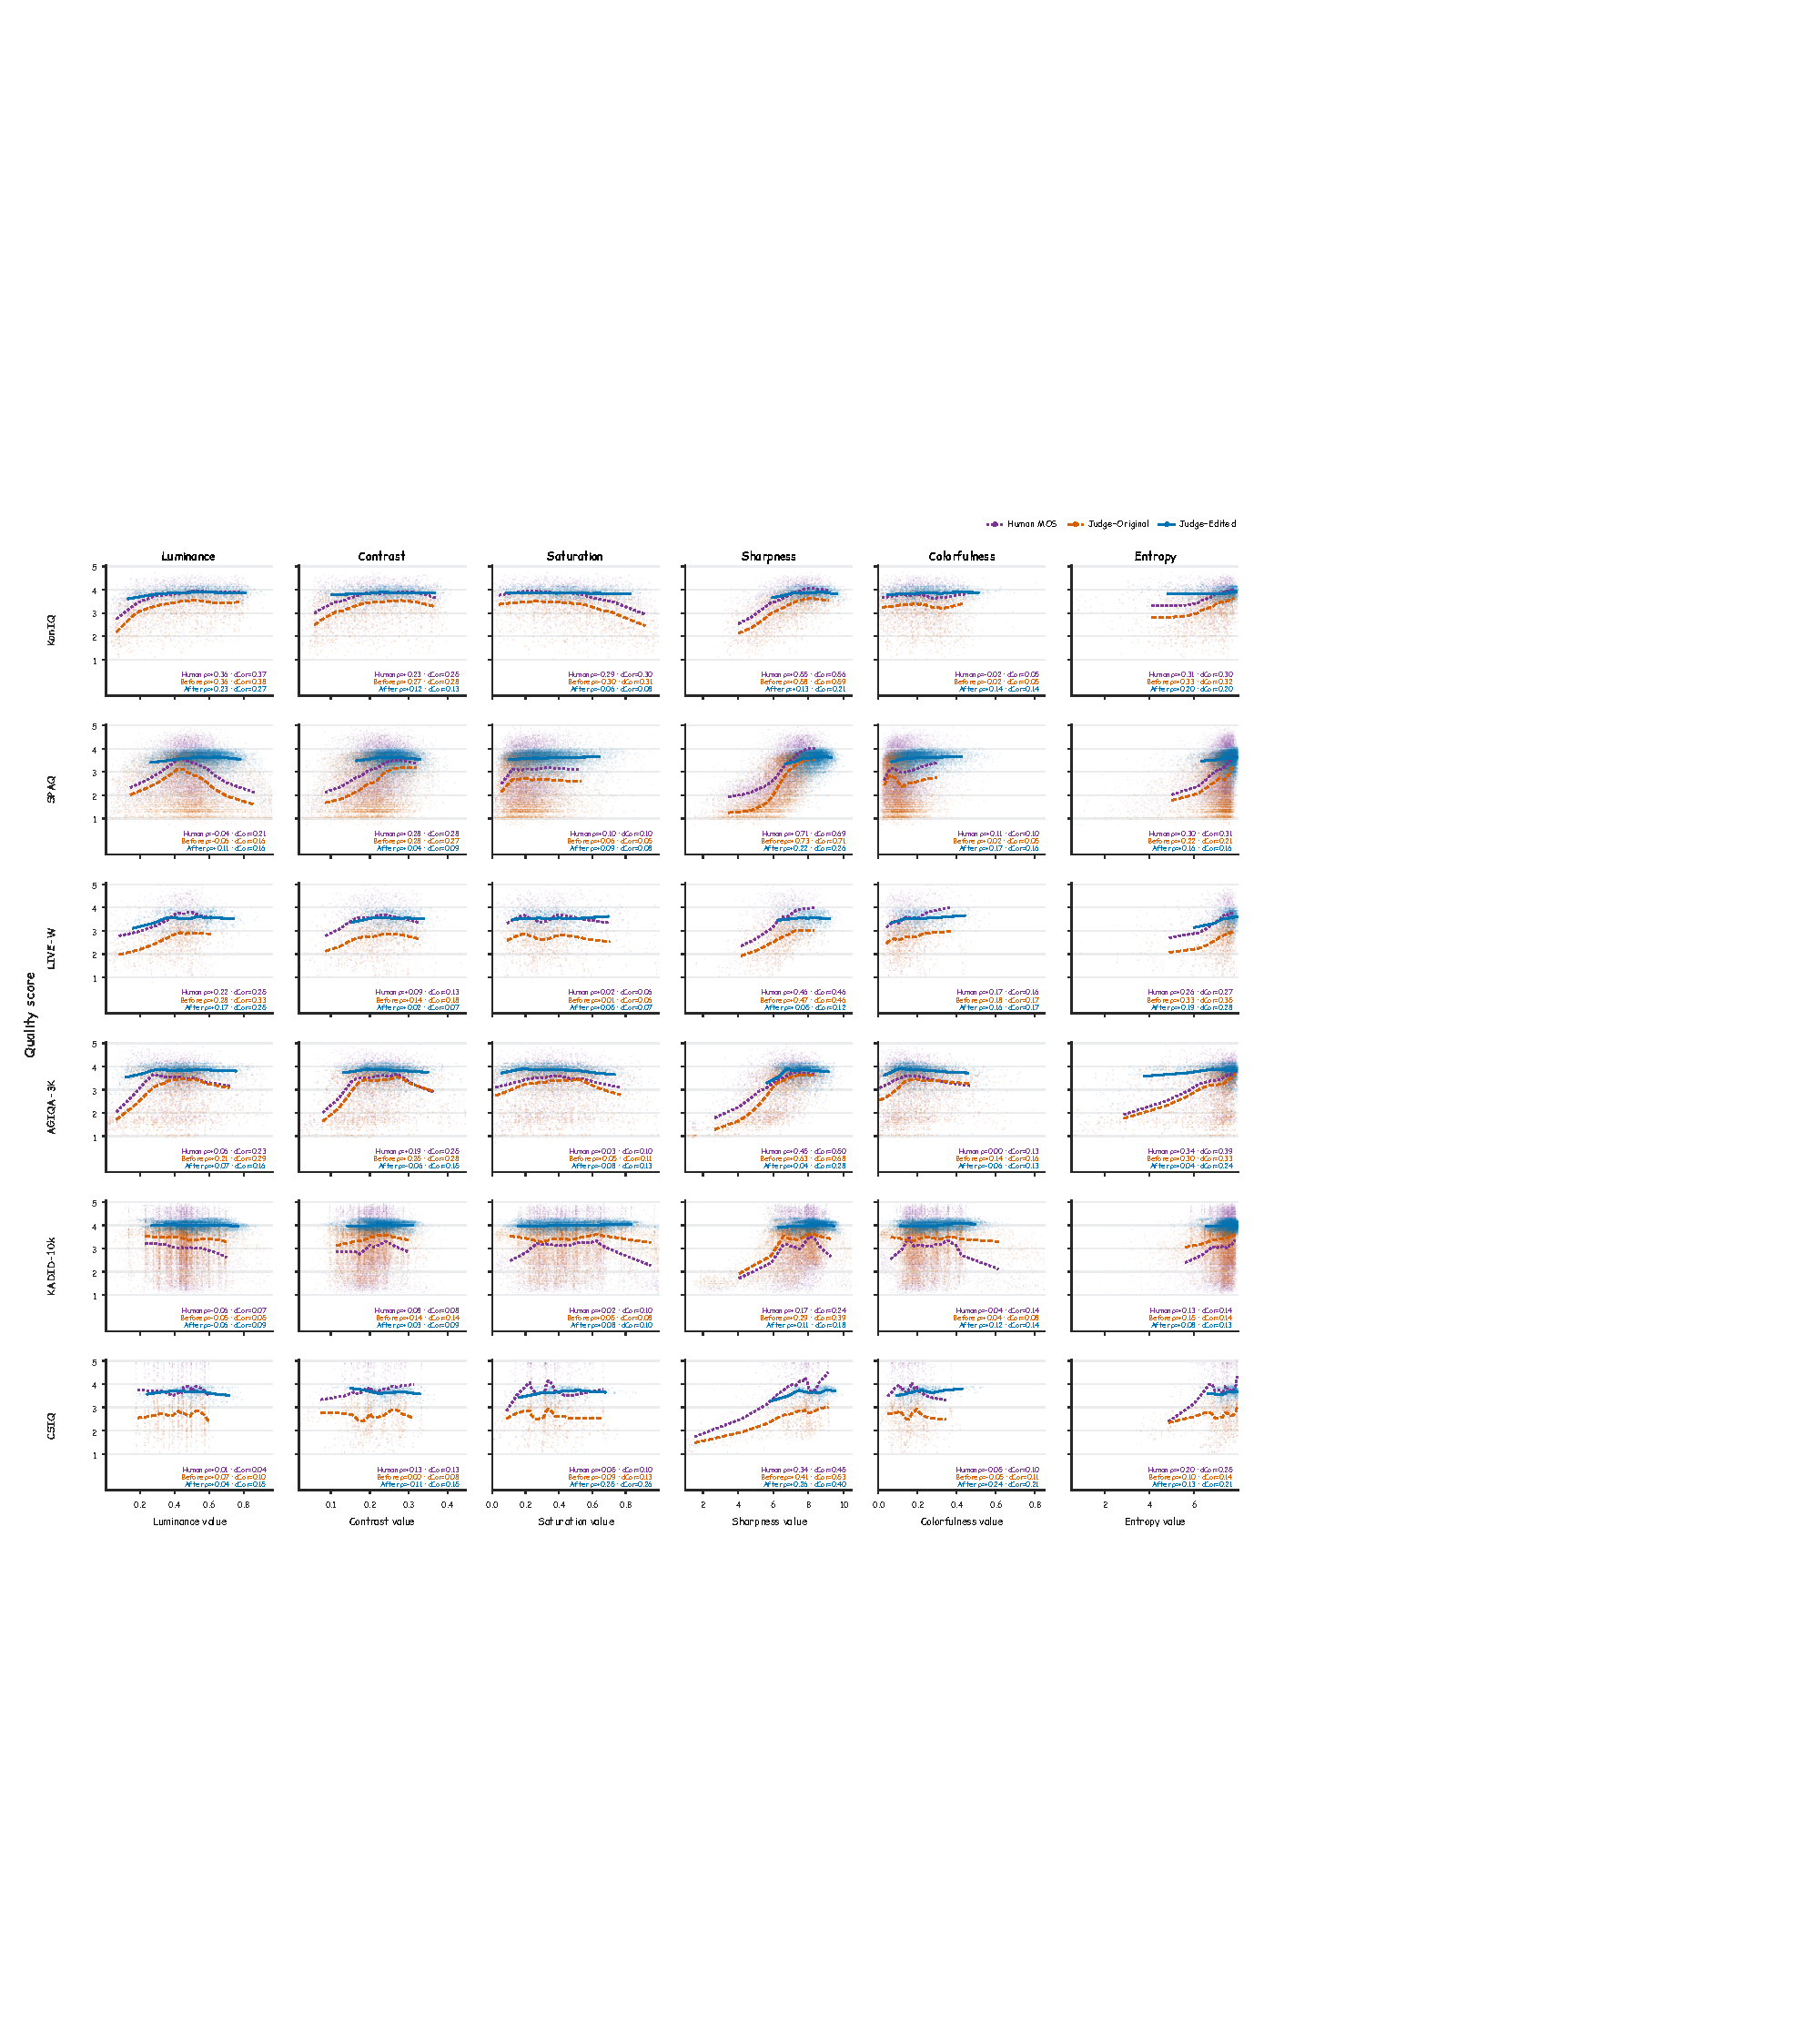
\includegraphics[width=\textwidth]{Figures/af1_figures_analysis.pdf}
\caption{\textbf{Quality scores versus low-level image features.} Rows denote
datasets and columns denote luminance, contrast, saturation, sharpness,
colorfulness, and entropy. Purple and orange show human MOS and Judge scores
for original images, while blue shows Judge scores for edited images. Curves
show smoothed trends; $\rho$ and dCor denote Spearman and distance
correlations~\citep{szekely2007distance}.}
\label{fig:quality-low-level-features}
\end{figure*}

\paragraph{Human-like Judge feedback.}
Figure~\ref{fig:quality-low-level-features} shows that the feature-dependent
curves produced by the original-image Judge broadly follow the corresponding
human-MOS curves across the six datasets. Their similar shapes and directions,
particularly for sharpness and contrast, indicate that the Judge captures
human-like quality preferences over low-level visual attributes. This
agreement supports its use as a qualified source of human-like feedback for
the original--edited image pairs.

\paragraph{Cross-dataset feature patterns.}
Among luminance, contrast, saturation, sharpness, colorfulness, and entropy,
sharpness exhibits the clearest cross-dataset trend. Both human MOS and Judge
scores generally increase with sharpness, whereas the other attributes show
weaker, nonlinear, or dataset-dependent patterns. This result suggests that
sharpness is a broadly shared quality cue, while no single low-level attribute
fully explains perceptual quality across all datasets.

\paragraph{Edited-feature distributions.}
After editing, the images retain broad distributions across all six low-level
attributes rather than collapsing to fixed feature values. The framework
therefore does not appear to overfit a single low-level pattern when improving
image quality. Nevertheless, Figure~\ref{fig:quality-low-level-features}
examines each attribute marginally. The joint distribution of low-level
attributes, and its relation to the human visual system and learned perceptual
representations such as CLIP-IQA~\citep{wang2023exploring}, warrants further
investigation.

\subsection{Framework Behavior Preference}

\begin{figure*}[p]
\centering
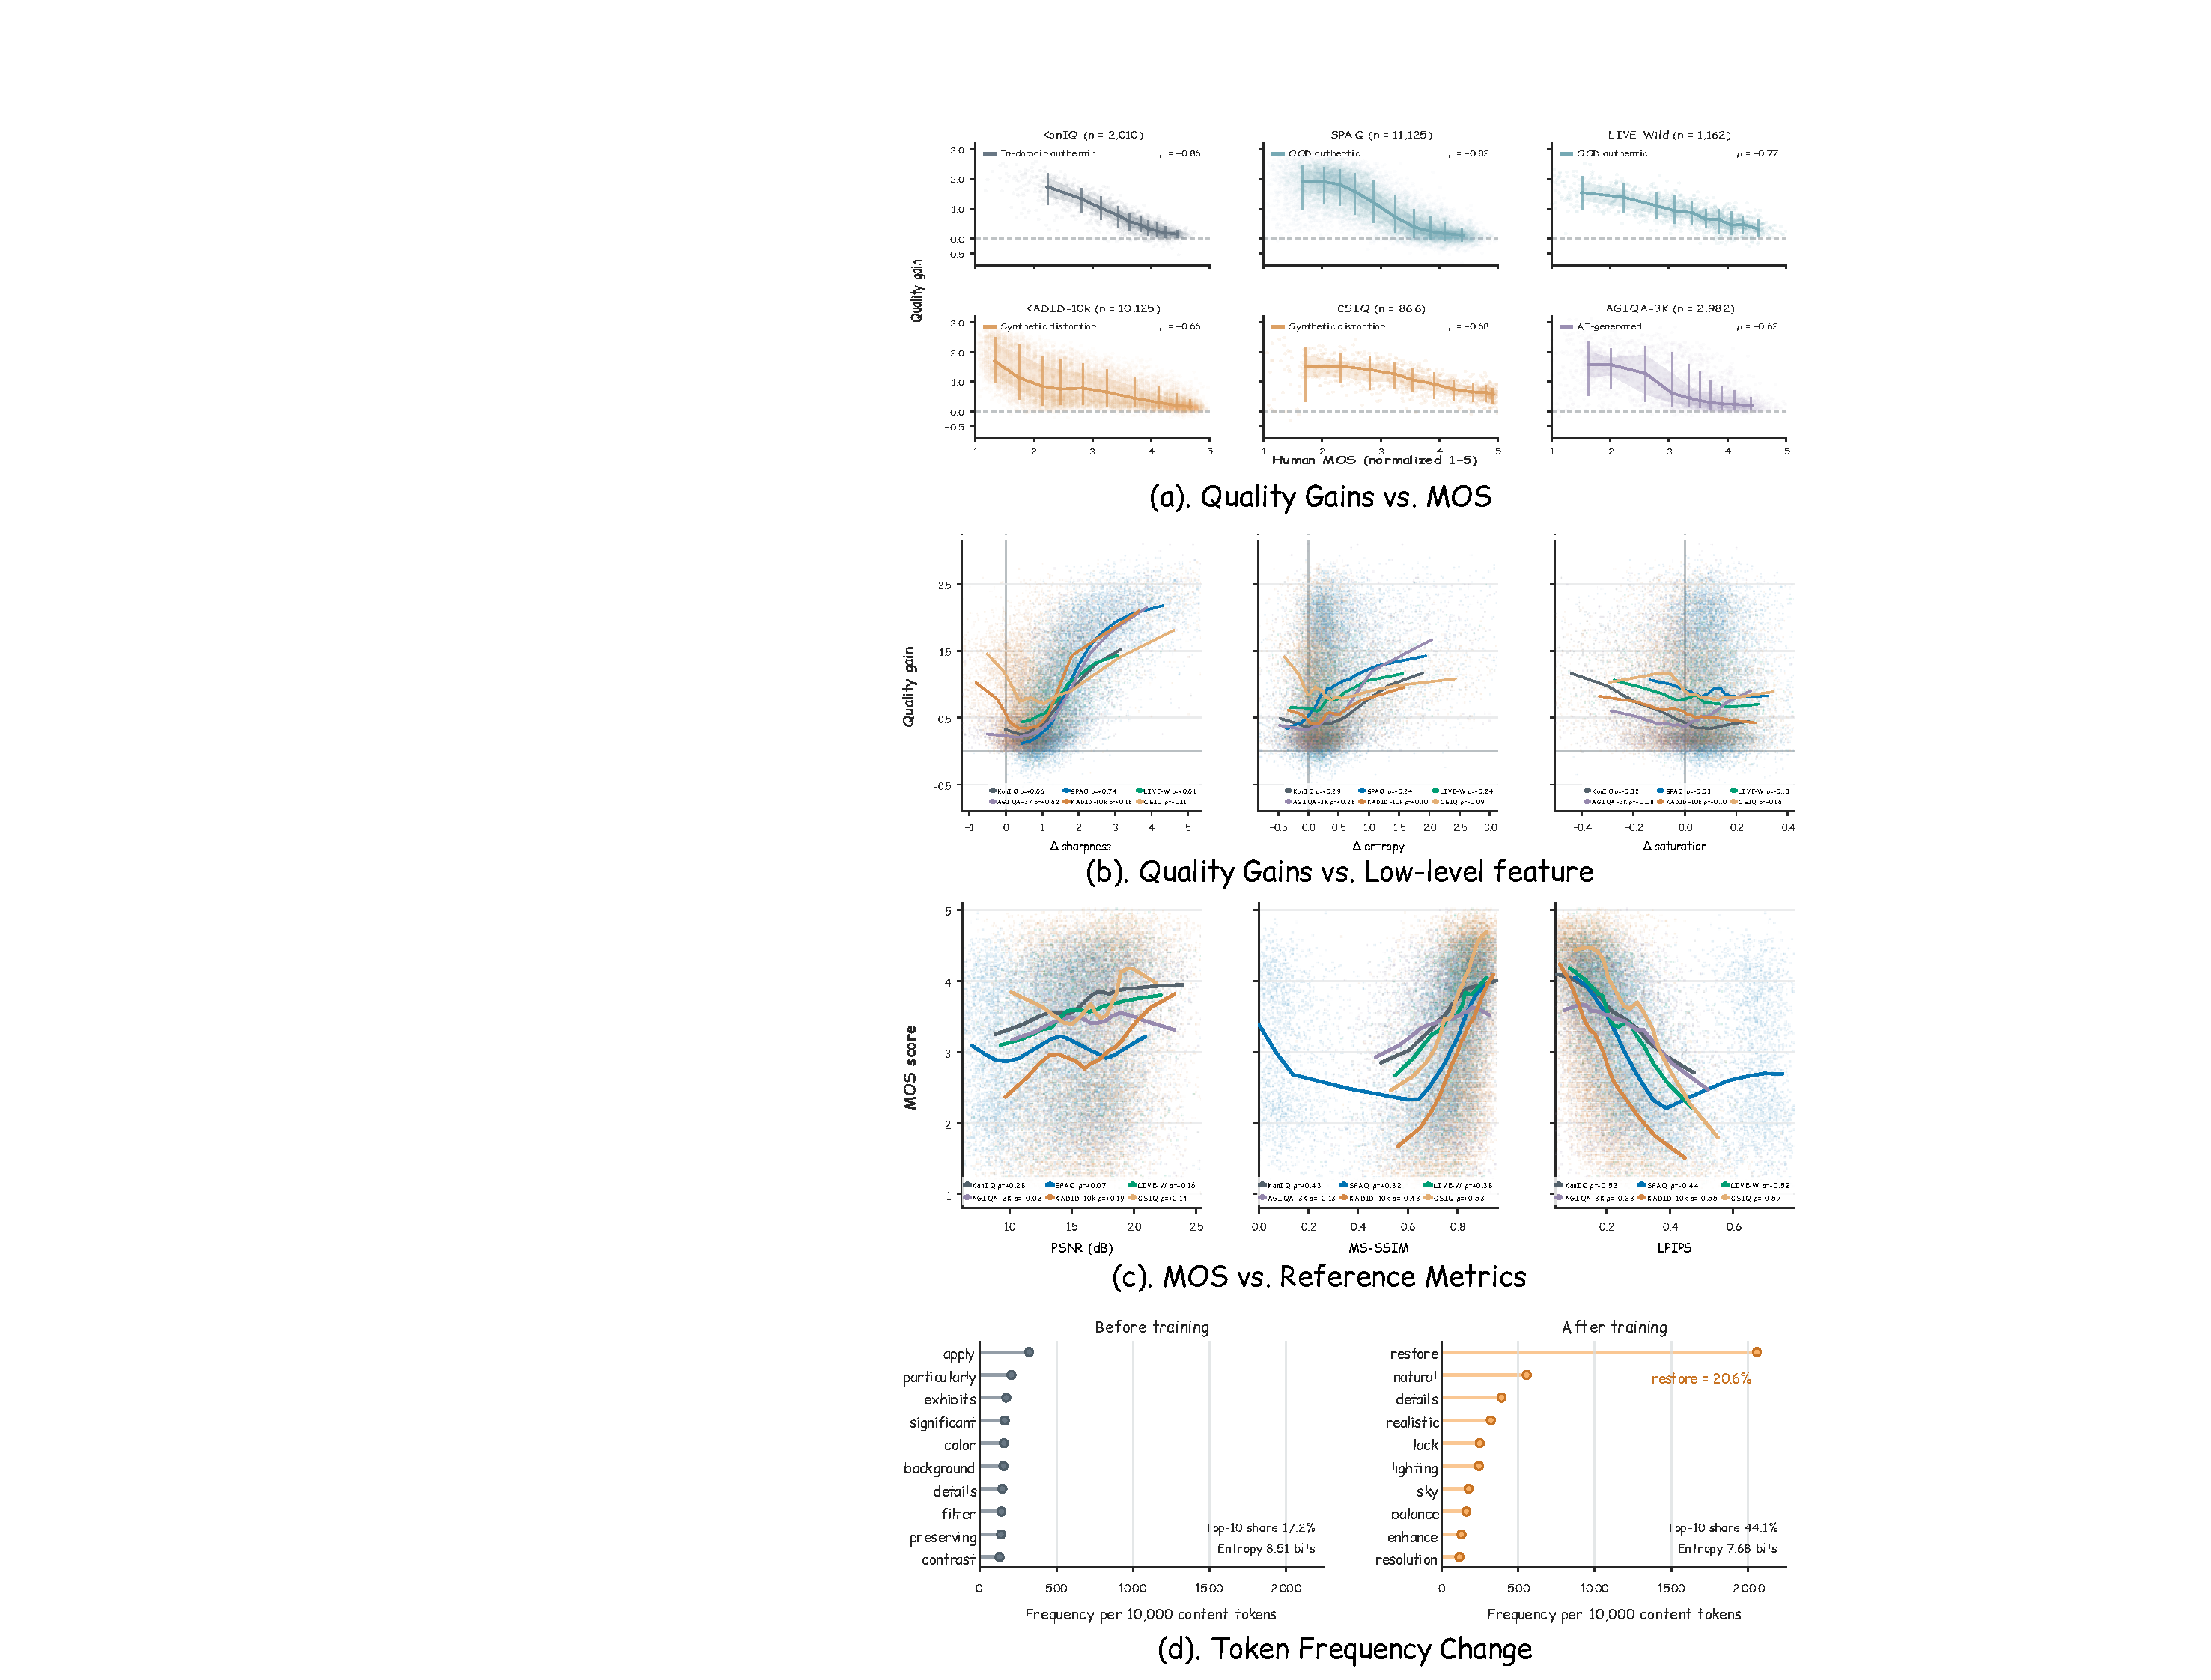
\includegraphics[
    height=0.90\textheight,
    keepaspectratio,
    pagebox=cropbox
]{Figures/af_4_figures_analysis.pdf}
\caption{\textbf{Behavioral analysis of reasoning-guided editing.}
(a) Judge-rated quality gain versus human MOS across six benchmarks.
(b) Quality gain versus changes in low-level image features.
(c) Human MOS versus reference-based similarity metrics between the original
and edited images.
(d) Frequent reasoning tokens before and after training.}
\label{fig:feature-analysis}
\end{figure*}

\paragraph{Source quality, visual change, and quality gain.}
Figure~\ref{fig:feature-analysis}(a) shows that lower-MOS images generally
receive larger Judge-rated quality gains. Panel (c) further shows that
lower-MOS images tend to have lower similarity between the original and edited
images, indicating larger visual changes. Together with the observation in
Section~\ref{app:quality-fidelity} that larger visual changes are associated
with higher quality gains, these results suggest a plausible behavior:
for lower-quality inputs, the model tends to modify more visual attributes,
which in turn leads to greater quality improvements. This behavior aligns with
the intuition that lower-quality images provide more room for correction and
supports the intended operation of our framework, although the observed
associations do not by themselves establish causality.

\paragraph{Preferences over feature changes.}
Unlike Section~\ref{app:quality-low-level-features}, which examines the
absolute values of low-level attributes, Figure~\ref{fig:feature-analysis}(b)
relates their changes after editing to the resulting quality gain. Changes in
sharpness retain the strongest and most consistent relationship with quality
improvement. For entropy and saturation, the authentic and synthetic datasets
form different response patterns, indicating that the preferred corrections
depend on the degradation domain. SPAQ again exhibits signals that are less
consistent with the other datasets, in agreement with the dataset-specific
behavior observed in Section~\ref{app:quality-fidelity}.

\paragraph{Behavioral adaptation and concentration.}
Figure~\ref{fig:feature-analysis}(d) reflects how the model adjusts its
reasoning vocabulary in response to Judge feedback. After training, terms such
as \emph{natural} and \emph{realistic} become prominent, revealing a learned
preference for perceptually plausible corrections. At the same time,
\emph{restore} alone accounts for 20.6\% of the displayed token frequency, and
the top-10 token share rises to 44.1\%. This concentration suggests an emerging
tendency to overfit a small set of solution patterns, despite the broader
behavioral alignment induced by the framework.

\section{Discussion on the Editor Proxy}
\label{app:editor-proxy}

This work does not disentangle the Editor's instruction-following capability
from semantic preservation, creating two attribution risks. First, quality may
degrade because of Editor limitations rather than an incorrect Actor
instruction. Second, the edited image may become semantically inconsistent
with the input, weakening quality change as a proxy for reasoning faithfulness.
Future work should use independent human or human-like evaluation to assess
instruction following, semantic consistency, and perceptual quality
separately, yielding more reliable feedback and a more faithful framework.

\iffalse
% Temporarily omitted from the supplementary material.
\begin{table*}[t]
\centering
{\small
\setlength{\tabcolsep}{3pt}
\renewcommand{\arraystretch}{0.96}
\begin{tabular}{@{}p{0.13\textwidth}p{0.24\textwidth}p{0.25\textwidth}p{0.33\textwidth}@{}}
\toprule
\textbf{Failure} & \textbf{Diagnostic evidence} & \textbf{Root cause} &
\textbf{Corrective measure} \\
\midrule
{\raggedright Edit-action collapse\par} &
Rating accuracy remained high, but every action was \texttt{no\_edit};
homogeneous six-sample groups had zero advantage. &
Within-group normalization cannot correct a homogeneous action and therefore
starves downstream edit-gain credit. &
Add counterfactual negative credit and low-quality resampling. Because edit
behavior did not recover, disable editing in the controlled actor-only
experiments. \\
\addlinespace[1pt]
{\raggedright Rating drift and invalid output\par} &
Ratings collapsed to 5.283 or shifted to 8--9.45 while pairwise ordering
remained informative. &
Reward parsing and validation used inconsistent validity rules. A pairwise
objective is also invariant to a global rating shift. &
Use one strict rating-range contract without reward-side clamping. Reject
invalid outputs and apply an absolute anchor only to homogeneous error groups. \\
\addlinespace[1pt]
{\raggedright Token-credit drift\par} &
Decoding and re-encoding generated IDs changed tokenization and shifted the
supervised field span. &
\texttt{encode(decode(ids))} is not guaranteed to reproduce the sampled token
sequence. &
Project field spans onto the original generated-token boundaries and use
prefix decoding only as a fallback for byte-split Unicode tokens. \\
\addlinespace[1pt]
{\raggedright Reward-variance collapse\par} &
1,513 of 1,536 groups had zero reward variance; only 138 of 9,216 completions
carried usable group advantage. &
Late-stage outputs became homogeneous. Additional sampling rounds did not
recover enough informative groups. &
Cap resampling, retain every complete effective group, and use complete
no-advantage groups only as zero-weight shape padding. Report effective-group
statistics explicitly. \\
\addlinespace[1pt]
{\raggedright Distributed underfill\par} &
With 282 effective rows, only one rank inserted padding and the distributed
token counts disagreed (7,046 versus 7,210). &
A rank-local predicate controlled a globally shared shape and normalization
path. &
All-reduce padding counts before branching, then execute the same physical-batch
and effective-token normalization path on every rank. \\
\addlinespace[1pt]
{\raggedright Schema and evaluation drift\par} &
Valid two-field outputs were parsed with an obsolete three-field schema; an old
SPAQ evaluation parsed only 34.07\% of ratings. &
Monitoring and evaluation did not share the schema, prompt, message template,
and backend used during training. &
Read schema from recorded trajectories and configuration, align the inference
contract with training, and report coverage together with PLCC, SRCC, and MAE. \\
\bottomrule
\end{tabular}
}
\caption{Method-relevant training failures and corrective measures. Values are
observed diagnostics, not benchmark results.}
\label{tab:training-failures}
\end{table*}

\FloatBarrier
\section{Technical Reports of Training Failures}
\label{app:training-failures}

\paragraph{Residual Limitation.}
The no-edit state remains unresolved: counterfactual credit was directionally
correct in 403 of 408 low-quality cases, but editing did not recover. Actor-only
ablations therefore omit editing and do not validate the full framework.
\fi

\FloatBarrier
\begin{figure*}[!t]
\centering
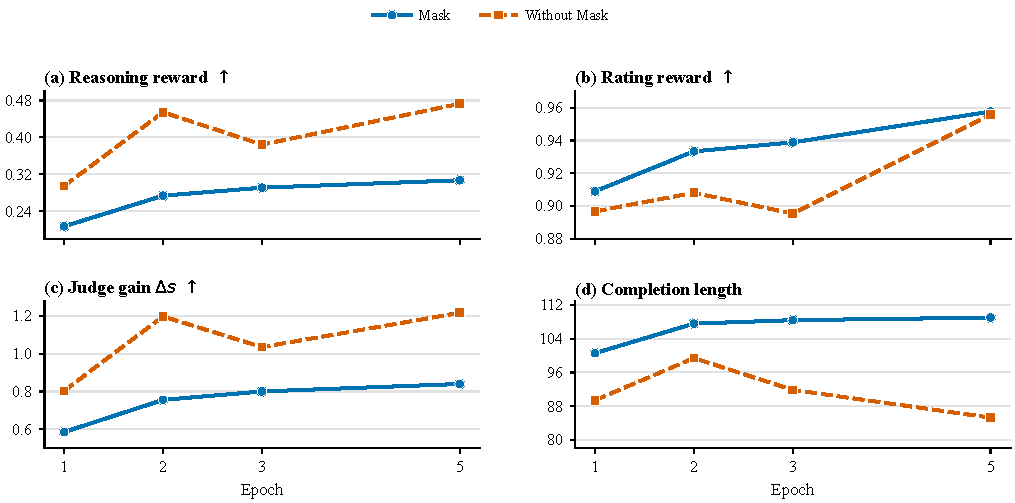
\includegraphics[width=0.85\textwidth]{Figures/fig_completion_audit_training.pdf}
\caption{\textbf{Training dynamics at the retained checkpoints.} Each point is
the exact four-rank mean for E1, E2, E3, or E5. Without Mask produces larger
reasoning reward and Judge gain, whereas rating reward converges similarly.
Its concurrent reduction in completion length is consistent with convergence
toward a high-reward solution template.}
\label{fig:credit-mask-training}
\end{figure*}

\section{Detailed Credit-Mask Audit}
\label{app:credit-mask-audit}

\subsection{Audit Scope and Protocol}
We audit two complete five-epoch runs with the same Actor, data, prompt, and
GRPO settings. \textbf{Mask} routes each reward to its supervised output with
output-specific KL regularization; \textbf{Without Mask} broadcasts rewards
over the complete output with one global KL term. Both use a KL coefficient of
$0.02$. The diagnostic reasoning reward bounds the raw Judge-score change:
\begin{equation}
    R_{i,k}^{\mathrm{diag}}
    =\operatorname{sgn}(\Delta s_{i,k})
    \left(1-\mathrm{e}^{-\Delta s_{i,k}^{2}/2}\right).
    \label{eq:diagnostic-reasoning-reward}
\end{equation}
The Editor consumes only the solution without an explicit semantic guardrail.
Both runs use six samples per image, 160-token completions, and frozen vision
encoder and aligner. Each contains 1,455 steps with 144 trajectories per step
(209,520 per run; 419,040 total). No step or record is missing, duplicated,
invalid, or non-finite. At Without Mask steps 711 and 713, all samples are
Actor-ineligible, so absent Judge changes reflect eligibility rather than
numerical or service failure. Because credit and KL routing change jointly and
each setting has one seed, this audit is descriptive rather than causal.

\subsection{Training Dynamics}
Figure~\ref{fig:credit-mask-training} reports exact four-rank means at the
retained checkpoints. Both configurations improve rating reward. Without Mask
produces larger reasoning reward and Judge gain, but also shorter outputs and
solution collapse. Mask changes more gradually: its reasoning reward rises
from 0.207 to 0.307 and Judge gain from 0.586 to 0.840. Rating rewards converge
by E5. KL losses are not directly comparable because their token scopes differ.
For Without Mask, mean reasoning reward and Judge gain increase from 0.463 and
1.189 over steps 1256--1355 to 0.478 and 1.232 over steps 1356--1455. Yet their
final-window slopes are $-0.0108$ and $-0.0246$; the rating-reward slope is
$-0.0006$. The endpoint therefore masks a plateau and slight decline.

\subsection{Checkpoint Validation}
Figure~\ref{fig:credit-mask-validation} evaluates the retained checkpoints on
the same 200 images. PLCC and SRCC improve for both runs. Without Mask keeps a
Judge gain near 1.18, while normalized-solution uniqueness falls from 91.88\%
at E1 to about 0.5\% at E2. The audit further shows that the semantic
dwelling-template rate reaches 100\% at E1. Semantic collapse therefore
precedes near-exact lexical collapse.

\begin{figure*}[!t]
\centering
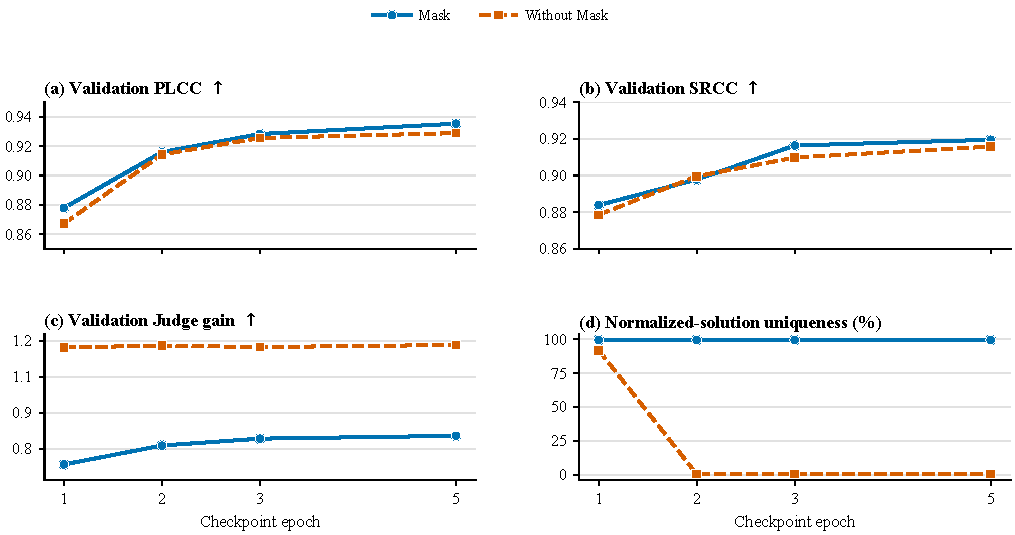
\includegraphics[width=0.85\textwidth]{Figures/fig_completion_audit_validation.pdf}
\caption{\textbf{Checkpoint validation dynamics.} Panels (a)--(c) report
PLCC, SRCC, and Judge gain on the complete 200-image validation set. Panel (d)
reports normalized-solution uniqueness. Without Mask maintains rating alignment
and high Judge gain while its solutions collapse.}
\label{fig:credit-mask-validation}
\end{figure*}

\subsection{Cross-Dataset Outcomes}
At E5, Without Mask obtains a larger pooled quality gain than Mask
($1.431$ versus $1.071$), although their six-dataset PLCC/SRCC averages remain
close ($0.834/0.812$ versus $0.838/0.812$). Larger gain alone therefore does not
establish healthier reasoning. All 28,270 Without Mask outputs share one
normalized solution; Mask retains 23,457 among 28,044 successful outputs.

\subsection{Collapse Milestones}
Table~\ref{tab:completion-audit-milestones} distinguishes semantic,
phrase-level, and near-exact collapse. Under Without Mask, the semantic
dwelling family exceeds 90\% at step 265, whereas one normalized sentence does
not exceed 90\% until step 551. Duplicate matching would detect the failure 286
steps late. Mask avoids dwelling collapse, although its super-resolution and
smoothing phrase backbone remains above 90\% from step 407 onward.

\begin{center}
\begin{minipage}{\columnwidth}
\centering
{\scriptsize
\setlength{\tabcolsep}{2.5pt}
\begin{tabular}{@{}p{1.55in}rrl@{}}
\toprule
\textbf{Routing and detector}
& $\boldsymbol{\geq 50\%}$ & $\boldsymbol{\geq 90\%}$
& \textbf{Sustained} \\
\midrule
Without Mask: semantic dwelling & 236 & 265 & 948--E5 \\
Without Mask: strict target phrase & 356 & 475 & -- \\
Without Mask: modal normalized solution & 520 & 551 & 973--E5 \\
Without Mask: canonical sentence & 1,133 & 1,146 & -- \\
Mask: super-resolution + smoothing & 214 & 260 & 407--E5 \\
\bottomrule
\end{tabular}
}
\captionof{table}{\textbf{Collapse milestones in global optimizer steps.} Semantic
detectors identify shared concepts before normalized near-duplicate matching
identifies one sentence.}
\label{tab:completion-audit-milestones}
\end{minipage}
\end{center}

\subsection{Output-Length Evolution}
Panel (d) of Figure~\ref{fig:credit-mask-training} shows that the mean training
completion decreases from 89.39 to 85.26 tokens under Without Mask but rises
from 100.57 to 109.00 under Mask. On validation outputs, the corresponding
solution lengths change from 32.56 to 18.00 and from 37.85 to 50.94. The former
contraction is consistent with convergence to one reusable instruction.

\subsection{Rating and Diversity Diagnostics}
Without Mask retains a KonIQ PLCC/SRCC of $0.932/0.914$ despite solution
collapse. Ratings still vary: 2,009 of 2,010 complete JSON outputs are unique,
although all 2,010 solutions are identical after normalization. Rating
correlation and full-output uniqueness therefore miss solution collapse.
Evaluation must inspect the supervised output alongside image--solution
relevance and semantic preservation.

\subsection{Representative Validation Outputs}
The Without Mask E5 Actor produces different evidence and ratings for the
three examples, but all solutions normalize to one dwelling instruction.
Sample 1 still receives 0.865 reward because the fixed intervention raises the
Judge score from 2.37 to 4.37. Thus, the reward measures edited-image quality
without establishing source-image faithfulness.

\begin{center}
\begin{minipage}{\columnwidth}
\centering
{\small
\setlength{\tabcolsep}{5pt}
\begin{tabular}{@{}lrrrrr@{}}
\toprule
\textbf{Sample} & \textbf{Rating} & $\boldsymbol{J_0}$
& $\boldsymbol{J_1}$ & $\boldsymbol{\Delta s}$ & $\boldsymbol{R}$ \\
\midrule
1 & 1.68 & 2.37 & 4.37 & 2.00 & 0.865 \\
2 & 3.32 & 3.84 & 4.32 & 0.48 & 0.109 \\
3 & 2.65 & 3.02 & 4.36 & 1.34 & 0.593 \\
\bottomrule
\end{tabular}
}
\captionof{table}{Representative Without Mask validation outputs. Different evidence
and ratings lead to the same normalized solution.}
\label{tab:completion-audit-examples}
\end{minipage}
\end{center}

\subsection{Causal Scope}
The comparison changes credit and KL routing jointly with one seed per setting.
It establishes a reproducible failure mode for Without Mask/global KL, but not
the responsible change. Causal attribution requires a $2{\times}2$ grid of
Mask versus Without Mask and component versus global KL, with multiple seeds.

\FloatBarrier
